
\documentclass{article}
\usepackage[utf8]{inputenc}
\usepackage{graphics}

\title{Bangla Handwriting Character Recognition}
\date{May 2021}

\begin{document}

\maketitle
\section{About us}
Submitted by:
Group: EWUSP2021CSE47504

Name: MD. Rakibul Hassan Robin
ID: 2017-1-60-033

Name: Lamiya Simran Proma
ID: 2017-1-60-003

Name: Sabikun Naher
ID: 2017-1-60-020

Name: Mahfuza Alam Orony
ID: 2017-1-60-048


Submitted to:
Md Mahmudur Rahman
Department of Computer Science and Engineering

\section{Introduction}
Bangla handwriting character recognition has many academic and commercial interests but it becomes a challenge to get good performance due to the alignment and many of them are similar. Another challenge in handwritten character recognition is to deal with the enormous variety of handwriting styles by different writers [1]. Existing methods are used to distinct characters and their recognition. Recently, Convolutional Neural Network (CNN) is found efficient for handwritten character recognition [2]. 
In this paper, CNN models have been proposed for classifying Bangla Handwriting characters. By using the state-of-the-art convolutional neural network (CNN) models in this study we investigate HBCR. We will be working with EfficientNet and LeNet models which will be evaluated based on a Bangla alphabet dataset and showing the results of experimentation. Then we will be compared the results by the performance and accuracy rate of this models and can find out which model performance is good for HBCR. Our objective is to find out a better performed algorithm to detect Bangla handwriting character recognition using a program and an existing dataset.
There are many applications of HBCR, such as Bangla optical character recognition, national ID number recognition system, automatic license plate recognition system for vehicle and parking lot management system, post office automation and online banking etc [1]. Some works related to your problem. Therefore, it is very necessary that HBCR applications will be performed in a good rate. In this paper, our main purpose is finding out how we can get a better performance of recognizing Bangla handwriting characters as well as we will demonstrate the improvement in accuracy for Bangla handwritten characters with convolutional neural network.
	

\section{Methodology}

In our project, we use two types of convolutional neural network methods.
1.	LeNet
2.	EfficientNet
LeNet: LeNet is a convolutional neural network structure. In general, LeNet refers to LeNet-5 and is a simple convolutional neural network. Convolutional neural networks are a kind of feed-forward neural network whose artificial neurons can respond to a part of the surrounding cells in the coverage range and perform well in large-scale image processing.[3] 
The LeNet-5 means the emergence of CNN and defines the basic components of CNN. But it was not popular at that time because of the lack of hardware equipment, especially GPU(Graphics Processing Unit, a specialized electronic circuit designed to rapidly manipulate and alter memory to accelerate the creation of images in a frame buffer intended for output to a display device) and other algorithms, such as SVM can achieve similar effects or even exceed the LeNet.[4] 
Since the success of AlexNet in 2012, CNN has become the best choice for computer vision applications and many different types of CNN have been raised, such as the R-CNN series.[5] Nowadays, CNN models are quite different from Lenet, but they are all developed based on LeNet.
Features:
\begin{itemize}
\item 	Every convolution layer includes three parts: convolution, pooling, and nonlinear activation functions
\item 	Using convolution to extract spatial features (Convolution was called receptive fields originally)
\item 	Subsampling average pooling layer
\item     Tanh activation function
\item 	Using MLP as the last classifier
\item 	The sparse connection between layers to reduce the complexity of computation
\end{itemize}


\begin{figure}
\centering
 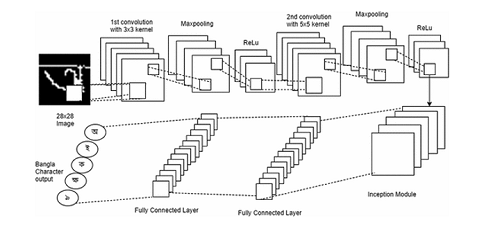
\includegraphics{fig.PNG}
\caption{ Diagram of LeNet method }
\end{figure}
   

                          
EfficientNet: EfficientNet is a convolutional neural network architecture and scaling method that uniformly scales all dimensions of depth/width/resolution using a compound coefficient  [6]. Unlike conventional practice that arbitrary scales these factors, the EfficientNet scaling method uniformly scales network width, depth, and resolution with a set of fixed scaling coefficients. EfficientNet uses a compound coefficient to uniformly scales network width, depth, and resolution in a principled way [7].
The compound scaling method is justified by the intuition that if the input image is bigger, then the network needs more layers to increase the receptive field and more channels to capture more fine-grained patterns on the bigger image.



\section{Implementation}

\subsection{Data Collection}
The text recognition system is trained on the Bangla character level by using a dataset named ‘Cmaterdb’ collected from google code archive [8]. We split this dataset into a small size dataset for processing the work faster. Our dataset has total 15001 handwritten character images. It consists of a sample of basic characters, and compound characters which are collected from the Bangla language. In Fig 1, the dataset provides multiple labels per character and group. It contains a variety of frequently used Bangla simple characters which is very complex shaped. 

\begin{figure}
\centering
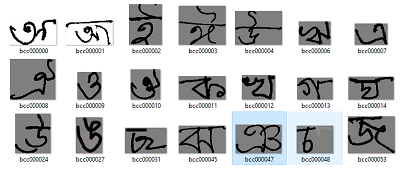
\includegraphics{image2.png}
\caption{Samples of Bangla handwritten characters}
\end{figure}
\subsection{Data Processing}
Duplicate data between training and test set can skew the results. So, we needed to remove all the overlap between training and test data. We used a fixed image size which is 64 × 64 pixels for each image. For resizing the images, we used the python imaging library pillow package which helped us to resize images easily.
\subsection{Model Development}
We used jupyter notebook to develop our program which is based on the python programming language. We used many of the python packages such as tensorflow, keras, pillow, numpy, etc. We have tried to train our model using tensorflow on two different algorithms, which were used to process and to work with handwritten image detection and recognition. For resizing images and processing images we used pillow package and for comprehensive mathematical functions, calculations we used numpy. The versions we used to develop for this project are python 3.7.9, tensorflow 2.4.0. We did rescaling, resizing 12000 images to 50 different classes and 3000 to another 50 different classes. We had 375 steps per Epochs and 50 Epochs and 93 validation steps to train our model for both of the algorithms. After training the model, the weights are saved to .h5 format.
\subsection{Results}
We have used two different algorithms to test our model for Bangla handwriting character recognition which is EffectiveNet and LeNet. 
    
    After using EffectiveNet our result is
    
loss: 0.0413 - accuracy: 0.9871 - val_loss: 0.1150 - val_accuracy: 0.9735

    After using LeNet our result is,
    
loss: 0.3223 - accuracy: 0.9047 - val_loss: 0.3789 - val_accuracy: 0.9032 .

Where our value is losing more in EffectiveNet and all the other results are quite similar. So we decided to use LeNet algorithm to use to run the project and check the success ratio. We tested the model several times and our average success rate is 80%
\section{Conclusions}
Here we have tried to recognize Bangla handwritten characters from various input sources or devices and came up with a solution to perform tasks simultaneously and efficiently[1]rtificial intelligence offers many benefits in pattern recognition and classification within the sense of copying human intelligence to a small extent. Handwritten character recognition is the first step to the vast field of Artificial Intelligence and Image Processing[1]
Convolutional neural network (CNN) is able to discover visual patterns directly from pixel images with a least prepossessing[2]. This investigates CNN structure without any feature selection for Bangla handwritten pattern classification [2]. We tested this method on a huge handwritten character dataset and compared the outcome with prominent methods for Bangla that is existing. The proposed method is shown competitive performance with the existing methods on the basis of test set accuracy but the proposed scheme seems efficient in size and computation. The presented result indicates that training of CNN might be improved and hence get better performance. Inspired by the human visual cortex CNN has the ability to recognize visual patterns directly from pixel images with minimal prepossessing.

\subsection{Challenges}
\begin{enumerate}
\item CNN structure is investigated without any feature selection for Bangla handwritten pattern classification. 
\item Here deep CNN architecture is robust in Bangla Handwritten Character Recognition but its dataset is huge[2]. 
\item No established method has been found where all the basic & compound characters are recognized with good accuracy[9].
\item The system is not working for a complete Bangla document. Characters must be written and processed separately
\end{enumerate}

\subsection{Limitations}


\begin{enumerate}
\item CNN structure is investigated without any feature selection for Bangla handwritten pattern classification. 
\item Here deep CNN architecture is robust in Bangla Handwritten Character Recognition but its dataset is huge. Also, we did not have a powerful graphics unit to train a huge dataset, so we had to split the dataset into a small part.
\item No established method has been found where all the basic & compound characters are recognized with good accuracy although we tried with two different algorithms.
\item The system is not working for a complete Bangla document. Only characters are being implemented on this project.
\end{enumerate}

\subsection{Future Scope}
There are tremendous scopes of future extensions of this work. Some of the scopes are listed out below: 
\begin{enumerate}
\item Multiple CNN channels (CNN ensemble) may be used to get majority based decisions. The expected error from the ensemble is always smaller than the expected error from a single predictor. 
\item Dropout layer may be introduced in the deep CNN model used in this work. Dropout is a regularization technique for reducing over fitting in neural networks by preventing complex co-adaptations on training data. 
\item Inception modules may be introduced. The idea of the inception layer is to cover a bigger area, but also keep a fine resolution for small information on the images. The idea is that a series of Gabor filters with different sizes will handle multiple object scales. With the advantage that all filters on the inception layer are learnable. The most straightforward way to improve performance on deep learning is to use more layers and more data. Study shows that incorporating Inception modules increases the accuracy rate. Google Net uses 9 Inception modules[10].
\item Residual Network layers may be introduced by feeding the output of two successive convolutional layers AND also bypass the input to the next layers. The idea of the residual network is to use blocks that reroute the input, and add to the concept learned from the previous layer. The idea is that during learning the next layer will learn the concepts of the previous layer plus the input of that previous layer. This would work better than just learning a concept without a reference that was used to learn that concept[5] .
\item The performance of the proposed CNN could be analyzed for Bangla compound characters and digits[2].
\item By using the OCR we can get the soft document of this data so that we can store this data and use it when it is needed or for an editable version. Day by day it will be made into a large dataset and the accuracy will be the highest accuracy for all the Bangla handwritten characters[11]
\end{enumerate}

 


\section{References}

\begin{enumerate}
\item M. Z. Alom, P. Sidike, M. Hasan, T. M. Taha, and V. K. Asari, “Handwritten Bangla Character Recognition Using the State-of-the-Art Deep Convolutional Neural Networks,” Comput. Intell. Neurosci., vol. 2018, 2018, doi: 10.1155/2018/6747098.
\item M. M. Rahman, M. A. H. Akhand, S. Islam, P. Chandra Shill, and M. M. Hafizur Rahman, “Bangla Handwritten Character Recognition using Convolutional Neural Network,” Int. J. Image, Graph. Signal Process., vol. 7, no. 8, pp. 42–49, Jul. 2015, doi: 10.5815/ijigsp.2015.08.05.
\item B. B. Chaudhuri & U. Pal. A complete printed Bangla OCR system. Pattern recognition.    1988.31.5:531-549p.
\item S. Afshar, G. Cohen and J. Tapson, A. Schaik. EMNIST: An extension of MNIST to  handwritten letters. arXiv:1702.05373[cs.CV], 2017.
\item D. Kingma and J. Ba, Adam: A method of stochastic optimization. arXiv:1412.6980[cs.LG], 2015.
\item R. Gonzalez and R.E. Woods. Digital Image Processing. Third Edition, 162-163p.
\item S. Afshar, G. Cohen and J. Tapson, A. Schaik. EMNIST: An extension of MNIST to handwritten letters. arXiv:1702.05373[cs.CV], 2017.
\item “cmaterdb.” 
https://storage.googleapis.com/google-code-archive-downloads/v2

/code.google.com/cmaterdb/CMATERdb3.1.3.3.7z (accessed May 20, 2021).
\item T. Ghosh, M. M. Abedin, S. Mahmud Chowdhury, and M. A. Yousuf, “A Comprehensive Review on Recognition Techniques for Bangla Handwritten Characters,” in 2019 International Conference on Bangla Speech and Language Processing (ICBSLP), Sep. 2019, pp. 1–6, doi: 10.1109/ICBSLP47725.2019.202051.
\item C. Xu, D. Chai, J. He, X. Zhang, and S. Duan, “InnoHAR: A Deep Neural Network for Complex Human Activity Recognition,” IEEE Access, vol. 7, pp. 9893–9902, 2019, doi: 10.1109/ACCESS.2018.2890675.
\item R. R. Chowdhury, M. S. Hossain, R. ul Islam, K. Andersson, and S. Hossain, “Bangla Handwritten Character Recognition using Convolutional Neural Network with Data Augmentation,” in 2019 Joint 8th International Conference on Informatics, Electronics & Vision (ICIEV) and 2019 3rd International Conference on Imaging, Vision & Pattern Recognition (icIVPR), May 2019, pp. 318–323, doi: 10.1109/ICIEV.2019.8858545.


\end{enumerate}







\end{document}
